\documentclass[tikz]{standalone}
\usepackage{pgfplots}
\pgfplotsset{compat=1.17}
\usetikzlibrary{shadings}

\begin{document}
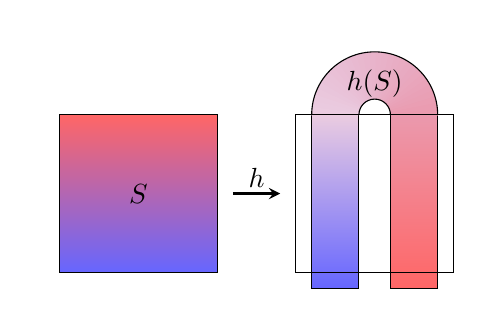
\begin{tikzpicture}
    \draw[white] (-0.4, -0.4) grid (5.1, 3.1);
    % \draw[help lines] (-0.1, -0.1) grid (5.1, 3.1);
    \draw[thick, -stealth] (2.2, 1.0) -- (2.8, 1.0); 
    \node at (2.5, 1.2) {$h$};
    % rectangle S
    \shade[bottom color=blue!60, top color=red!60] (0, 0) rectangle (2, 2);
    \draw (0.0, 0.0) rectangle (2.0, 2.0); 
    \node at (1, 1) {$S$};

    % horseshoe map
    \shade[bottom color=blue!60, top color=blue!40!red!20] (3.2, -0.2) rectangle (3.8, 2);
    \draw (3.2, -0.2) rectangle (3.8, 2.0); 
    \shade[bottom color=red!60, top color=blue!20!red!40] (4.2, -0.2) rectangle (4.8, 2);
    \draw (4.2, -0.2) rectangle (4.8, 2.0); 
    % half ring
    \newcounter{i}
    \setcounter{i}{1} % 1 始まりのカウンター
    \def\n{30} % 任意の n を指定
    % 多角形の各頂点を計算
    \foreach \k in {1, ..., \n} {
        \pgfmathsetmacro\theta{180/\n * (\k - 1) - 1.0}
        \pgfmathsetmacro\phi{180/\n * \k + 1.0}
        \coordinate (A\arabic{i}) at ({4.0+0.8*cos(\theta)}, {2.0+0.8*sin(\theta)}); 
        \coordinate (B\arabic{i}) at ({4.0+0.8*cos(\phi)}, {2.0+0.8*sin(\phi)}); 
        \coordinate (C\arabic{i}) at ({4.0+0.2*cos(\theta)}, {2.0+0.2*sin(\theta)}); 
        \coordinate (D\arabic{i}) at ({4.0+0.2*cos(\phi)}, {2.0+0.2*sin(\phi)}); 
        \stepcounter{i} % カウンター i を 1 増加
    }
    \foreach \x in {1, ..., \n} {
        \pgfmathsetmacro\b{20+\x*20/\n}
        \pgfmathsetmacro\r{40-\x*20/\n}
        \fill[color=blue!\b!red!\r] (A\x) -- (B\x) -- (D\x) -- (C\x);
    }
    \draw[] (4.8, 2.0) arc (0:180: 0.8);
    \draw[] (4.2, 2.0) arc (0:180: 0.2);
    % rectangle S
    \draw (3.0, 0.0) rectangle (5.0, 2.0); 
    \node at (4.0, 2.4) {$h(S)$};

\end{tikzpicture}
\end{document}